
\chapter{Methodology} \label{ch-2}

\begin{large}
	
This section describes the components and methodologies used to achieve the objectives defined in previous section. Since the chosen methodology is based on RL, which is a data-driven method that learns control action directly from the datasets using Deep Neural Networks(DNNs). It begins with descriptive analytics of dataset in use. The subsection following describes foundations and concepts of theoretical framework in use. The RL based framework requires trial and error learning, therefore there is need of implementation of custom environment simulating HEMS. The simulated environment and its different types, based on their involvement in steps of modeling are discussed. A reward function definition/design is crucial part of the setup to learn policy as the reward reinforcement dictates the behavior(action under given policy) of an agent. Finally appropriate algorithms are selected for the learning of the policy itself. \\ 


\section{Data Description}

Since the modeling of policy network or deep neural networks in general, is based direct mapping of data to resulting unit(action), it is important to select input observation/features to be representative of information needed by agent to make decisions. The dataset \cite{dataset} provided is an open dataset on residential bidirectional EV charging. It includes roughly a year of time series dataset with 15 minutes resolution, collected in private customer household in southern germany. The dataset includes power monitoring at Grid Connected Point(GCP) with positive values, generated PV power with negative values and power through bidirectional Electric Vehicle Supply Equipment(EVSE) as positive values. Power drawn by a household ($P_{HH}$) is derived as $P_{HH}=P_{GCP}-P_{PV}-P_{EVSE}$. It further includes information on EV such as boolean connection status, current State of Charge(SoC) of the EV and target SoC(SoC level to attain with user pre-defined departure time). Although the dataset is useful for many scenarios such as EV power exchange to Household, Grid, other Energy consumption devices, for the use case at hand, only the information on Power consumed from grid to meet household demand ($P_{HH}$), power of generated PV($P_{PV}$) is utilized. The unit of Power is measured in Watts. Additional time series dataset\cite{energychartsinfo} on day ahead variable energy exchange price of hourly resolution is utilized. \\

Further description of data is projected as distribution of samples for each selected features as shown in figure \ref{fig:dev_datainfo}. The distribution of sample values in Power PV data is shown in the upper left section of the figure. As discussed in the data collection process\cite{dataset}, the data values of ($P_{PV}$) is always below $0$. Around $64\%$ of the sample values lie within $(-0.5, 0)$ with average value of $-1.789$. Similarly, in the upper right section of the figure represents distribution of values for Power Household with $71\%$ of value within $(0, 0.5)$. These ($P_{HH}$) value have mean of $0.542$ and always lie above $0$. Auction price data is a near normal distribution with mean value of ($0.192$). These statistics could provide some insights on impact of set of these observation input values on resulting action of the Agent. \\


\begin{figure}[h]
	\begin{center}
		\includegraphics[width=0.9\textwidth]{development/input_distributions.png}
		\caption{ \textit{Data distribution of observation inputs} }
		\label{fig:dev_datainfo}
	\end{center}
\end{figure}

While distribution may provide information on individual samples, it fails to represent the temporal relationship among them. Upon additive decomposing, the data series can be visualized in terms of component such as Trend(T), Seasonality(S) and Residuals( i.e. $\text{Time Series}=T+S+R$). The Repetition of patterns of behaviors in household consumption and PV generation, reflected on different scale of time range are termed as seasonality. The trend component can be interpreted as margin of consecutive values over period of time or patterns without seasonal component. The residual part of the series, as the name suggests, is rest of the composition after reducing patterns of trend and seasonality. \\

Figures \ref{fig:dev_input_decompose_daily} and \ref{fig:dev_input_decompose_hourly} show decomposition of input observation series for a day in a week and hour in a day respectively. There are several scales of patterns that can be identified through the full range of dataset length such as season or months of the year with variation in PV generation, price of energy. Yearly and Monthly decomposition is limited by size of dataset. Selection of time frame window as day in a week allows us to see and compare daily pattern in consumption shown in blue graph in upper left section. It starts with Friday with heavy consumption pattern during morning and evening hours, higher during weekends and average for the rest of the weekdays. A trend in increase in auction price can be seen during weekdays and reduced in weekend likely reflection of less demand from industries.  \\

\begin{figure}[h]
	\begin{center}
		\includegraphics[width=0.9\textwidth]{development/input_daily_decomposition.png}
		\caption{ \textit{Additive decomposition of observation inputs (daily)}}
		\label{fig:dev_input_decompose_daily}
	\end{center}
\end{figure}

Since the PV patterns are independent of weekdays, an hourly decomposition in a day was selected as shown by the green curve. The PV peaks during mid-day when the sun is up, household demand is less during work hours. \\

\begin{figure}[h]
	\begin{center}
		\includegraphics[width=0.9\textwidth]{development/input_hourly_decomposition.png}
		\caption{ \textit{Additive decomposition of observation inputs (hourly)} }
		\label{fig:dev_input_decompose_hourly}
	\end{center}
\end{figure}

The description of different properties of dataset such as sample distributions, seasonal and trend components decomposition could allow interpretation of the pattern in agents behavior later during inference, since these input series solely are used to learn policies. The residual part is distinguished from other component and may represent important information whereas seasonality and trend might introduce fluctuations. \\

\section{Theoretical Framework}

Main concept of reinforcement learning (RL) revolves around an agent learning to make decisions in an environment through trial and error, with the goal of maximizing a reward. A typical agent environment interaction\cite{rlintro} is shown in the figure \ref{fig:fmdp}. The main components and terminologies of such interactions are described as follows.\\


\begin{figure}[h]
	\begin{center}
		\includegraphics[width=0.8\textwidth]{components/finite_mdp.png}
		\caption{ \textit{Agent environment interaction}}
		\label{fig:fmdp}
	\end{center}
\end{figure}


\begin{itemize}
	\item{\textbf{Environment}: It is the world or system the agent operates in. It provides the agent with feedback in the form of rewards or penalties based on its actions.}
	\item{\textbf{State}: It represents the current situation in the environment relevant to the agent's decision-making. Special states are initial and termination states}
	\item{\textbf{Reward}: It is a numerical value assigned to the agent after it takes an action. Positive rewards indicate good choices, while negative rewards indicate bad choices. The reward function guides the agent's learning by shaping its understanding of what actions lead to intended behavior.}
	\item{\textbf{Policy}: It is the strategy the agent uses to map states to actions. Through trial and error, the agent learns and refines its policy to make better decisions in the future. The cycle of action, reward, and policy update continues as the agent learns through experience until some termination or truncation criteria is met.}
	\item{\textbf{Action}: It is what the agent chooses to do in a particular state under current policy/rule.}
\end{itemize}

A RL system in context of HEMS with finite set of observation states is based on a decision process termed as Markov Decision Process(MDP) and is defined in terms of tuple $(S, A, P, R, \gamma)$. where, $S$ is set of all possible permutation of observation values, $A$ is set of all possible action taken by decision making agent, $P$ is state transition probability matrix $P_{ss^{'}}^{a}$ as state transition to future state $S_{t+1}$, given current state $S_t$ for current action, i.e. $P_{ss^{'}} = \mathbb{P}[S_{t+1} = s^{'} | S_t = s]$, $R$ is estimated return $R_{s}^{a} = \mathbb{E}[R_{t+1} |S_{t}=s, A_{t}=a]$ given state and action pair, $\gamma \in [0,1]$ is a discount factor that defines the relevance of future returns on computing the current reward i.e. if $\gamma =1$, no discounting and if $\gamma=0$, only considering the next consecutive reward $R_{t+1}$. \\


\section{Custom HEMS Environment}

In order for a learning system to work on different set of input observation and resulting action, a simulated household environment is to be implemented, which is safer and efficient than a real world scenario. \\

\begin{figure}[h]
	\begin{center}
		\includegraphics[width=0.8\textwidth]{components/custom_env.png}
		\caption{ \textit{Custom simulated HEMS environment} }
		\label{fig:custom_env}
	\end{center}
\end{figure}

A customized HEMS environment is setup using \cite{gymnasium} as shown in the figure \ref{fig:custom_env}. It consists of an integration of a energy storage(EV or Home battery), with current state of it's content, used as part of input observation and updated with the subsequent actions depending on whether the action is to charge and discharge from the battery respectively. The action taken by an agent is modeling of charging and discharging power $P$ (kW) of bi-directional battery charger/EVSE. A small update in battery energy content $\Delta \text{SoC}$ is formulated based on pre-defined range of action space and battery capacity as given by equation \ref{eq:socdelta}. \\


\begin{equation}
	\boxed{
		\Delta \text{SoC} = \frac{\eta \times P \times dt}{C} 
	}
	\label{eq:socdelta}
	\tag{1}
\end{equation} \\


where, $\eta$ is Columbic efficiency accounting energy losses during charging or discharging, $C$ is battery capacity (kWh), and $dt$ is a small change in time (hours) for soc update. The energy content is therefore updated based on power flow direction $\pm P$ as shown in equation \ref{eq:socupdate} \\

\begin{equation}
	\boxed{
		\text{Updated SoC}  = \text{Current SoC} + \Delta \text{SoC} 
	}
	\label{eq:socupdate}
	\tag{2}
\end{equation} \\

Based on the functionality, a custom HEMS environment is initialized with different set of parameters to train, evaluate and test given policy as shown in figure \ref{fig:env_types}. The training environment is initiated with part of train set input observation and wrapper to facilitate vectorization depending on number of environments in use. A separate evaluation environment is to be initiated to evaluate current policy after $i$ number of training iteration and parameter updates in policy network. The evaluation environment is wrapped for monitoring to log information during policy evaluation-improvement iteration. Finally, to assess the policy on unseen observation, a test environment is initialized with test set of observation and respective parameters. \\

\begin{figure}[h]
	\begin{center}
		\includegraphics[width=0.8\textwidth]{components/env_types.png}
		\caption{ \textit{Types of environments}}
		\label{fig:env_types}
	\end{center}
\end{figure}


\section{Reward Function Definition}

Definition and design of reward function is at the core of modeling agents behavior. For each step in an environment, agent is encouraged for desirable action and vice-versa. For the use case at hand, the desirable actions are defined in terms of minimizing net household exchange cost to the grid, i.e. optimizing household total energy cost. An additional objective of retaining fraction of energy content could be introduced, in case of emergency Household or EV usage in combination with minimizing energy cost. This combined formulation of rewards adds a layer of complexity but optimizes multiple objectives. \\

The reward function used to optimize net exchange cost of a household, computed as primary objective, is given by the equation \ref{eq:costreward}. It serves as primary objective of this undertaking \\


\begin{equation}
	\boxed{
		\textbf{cost reward} = \left(\text{power household} + \text{power pv} + \text{action}\right) \times \text{auction price}
	}
	\label{eq:costreward}
	\tag{3}
\end{equation} \\

Combination of the primary reward with soc retain as secondary objective is defined in equation \ref{eq:combinedreward} to explore optimization of multiple/combined objectives.

\begin{equation}
	\boxed{
		\textbf{combined reward} = \text{net exchange cost} \pm \text{soc retain reward} 
	}
	\label{eq:combinedreward}
	\tag{4}
\end{equation} \\

Where, $\text{soc retain reward} = +0.25$ for battery SoC to stay above defined threshold of $0.45$ and $-0.25$ otherwise. The number $0.25$ is chosen as a better value among values after several trial and improvement within range of $(0.1, 1)$. Since finding the right value in combined reward is a trade-off between constituent rewards, before this value there were no visible improvement in soc baseline. This trade-off is discussed in the supplementary observation section \ref{ch-6}. 

\section{Algorithm Selection}

Selecting an algorithm appropriate for modeling of the policy based on the custom environment, considering type of action and observation spaces, availability of information on dynamics of the environment and types of learning is key step to modeling Prosumer Agent. Figure \ref{fig:algorithm_selection} shows classification of algorithms based on these criteria. \\


\begin{figure}[h]
	\begin{center}
		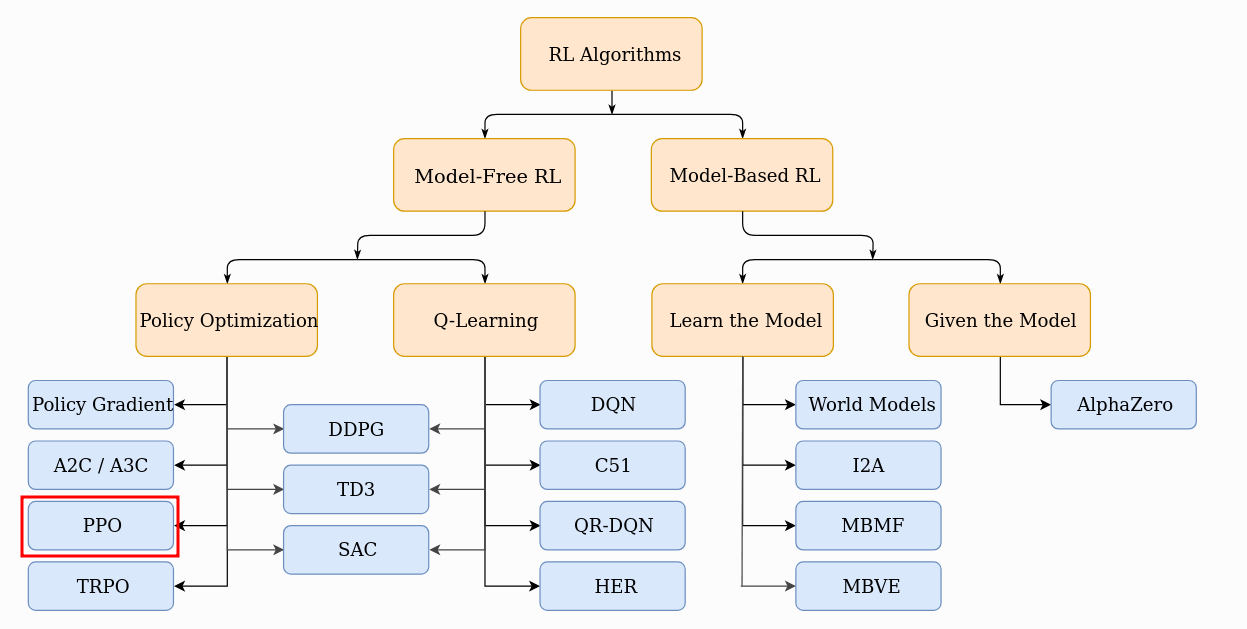
\includegraphics[width=0.8\textwidth]{components/algorithm_selection.png}
		\caption{ \textit{RL algorithm classification} src: \cite{openaispin}}
		\label{fig:algorithm_selection}
	\end{center}
\end{figure}


As mentioned in custom environment section above, the action to be performed by an agent is the bidirectional charging and discharging power of a battery storage system on a continuous series of observation, an algorithm with continuous action space is selected. Based on policy learning type on whether to use the sample collection and simultaneous learning(i.e. on-policy) or to used sample collection and learn from them separately (i.e. off-policy), algorithms of both type were considered. \\


Based on state spaces exposed to the agent, the observable space is only partial. Since the full dynamics of environment are not known beforehand, model-free algorithms are considered for their simplicity and effectiveness. Considering above described criteria, policy gradient based algorithm Proximal Policy Optimization(PPO) \cite{ppo}, Soft Actor Critic(SAC)\cite{sac}, and Twin Delayed Deep Deterministic Policy Gradient(TD3)\cite{td3} were selected from \cite{sb3} for the experiments. \\

A partial but crucial component of the algorithm is an actor network that predicts action given the set of observation. The actor network is part of in each all the selected algorithms. A typical architecture of an actor network is shown in figure \ref{fig:actor_network}. Given observation inputs of Power household, Power PV, Energy exchange price and current battery SoC, action is the resultant of an Fully connected Multi Layer Perceptron(FC-MLP), with appropriate activation $Z$(hyperbolic tangent due to it's compatibility with action space $A \in [-1,1]$). \\

\begin{figure}[h]
	\begin{center}
		\includegraphics[width=\textwidth]{components/actor_network.png}
		\caption{ \textit{Actor (pi) network}}
		\label{fig:actor_network}
	\end{center}
\end{figure}


Modeling a Prosumer Agent for selected algorithms effectively for the application under consideration, evaluating performance and identifying different factors influencing the learning of better strategies is the main focus of this undertaking. The briefed methodologies above guide the development of experimental setup in the following section \ref{ch-3}. \\

To bring the components together, steps of procedure is to be outlined for development. Following the definition of custom environment and their types, selected algorithms, relevant system states are defined. An action boundary, constraining agents action to operational range of a battery system is to be setup. A mapping of system states to resulting action is in accordance with the selected algorithms for learning policies. Starting from randomly initialized policy and criteria defining reward estimation, an appropriate behavior is modeled via the interaction of environment and policy learning algorithms.  An agent is evaluated based on actions that optimizes the household net cost of exchange to a grid under variable tarrifs and improved based on the reward feedback. This iterative policy learning, evaluation and improvement process is expected to derive policy toward optimality. \\ 


\end{large}
% ------------------------------------------------------------------------------------
